\section{Introduction}

Since its discovery, the Dunhuang Grottoes have been an important site for the study of Buddhist art and
several important aspects of Chinese history, including the trade events via the Silk Road, etc.
While a large quantity of artefacts like the murals and sculptures have survived thousands of years
to be presented in this modern age, the artefacts are facing significant threats from various factors.
A study of \apaciteassub{Jiang2023-Weather-Dunhuang} has shown that the despite the lack of immediate risk
of preservation due to the drastic climate change in the past few decades, the artefacts are still
prone to deterioration due to the weathering effects of the natural environment. Therefore, the
preservation of the Dunhuang treasures is of utmost importance and a race against time
(\apaciteaspar{Yu2022-AI-Dunhuang}). Measures with high efficiency are needed to ensure the survival
of the cultural heritage.

In view of the above, the Dunhuang Research Academy (DHA) was established in 1944 and is now devoted to
applying modern technologies to the preservation of the Dunhuang Grottoes. While one takes advantage of
the efficiency and convenience of modern technologies, such as Artificial Intelligence (AI), one must
also be careful about the potential damages that may be imposed on the cultural heritage.
This essay aims to explore the current applications of the AI technology in the preservation of the 
Buddhist heritage, using the Dunhuang Caves as a case study. In the Literature Review section, some
cutting-edge AI applications in the archaeological field will be briefly explored. Then, in the
following two sections, the benefits and potential risks of these applications will be discussed.
Finally, a conclusion on the topic will be included, with a hope that the discussion would provide new
insights into the process of critically evaluating the use of AI in the preservation of cultural heritage.

\subsection{Terminology}

Since the topics ``cultural heritage'', ``preservation'' and ``AI'' are all broad, it may be helpful if
these terms are defined before the discussion commences. 

\subsubsection{Buddhist Heritage and Cultural Heritage}

In the context and the scope of discussion of this essay, the term ``Buddhist heritage'' and ``cultural
heritage'' are treated as the same, and they refer to both the artefacts and sites of the Dunhuang Grottoes.
The ``artefacts'' include the mural paintings, sculptures, manuscripts that were recovered from the Library
Cave (Cave 17) and other caves. The ``sites'' refer to the region, and the caves' architectural and structural
designs and features. This definition is consistent with that of the current standard as suggested by
\apaciteassub{UNESCO2024-Cultural-Heritage}.

\subsubsection{Preservation}
\label{sec:preservation-definition}

As suggested by \apaciteassub{UNESCO2024-Conservation}, the conservation and preservation of cultural heritage
are means taken to elongate the lifespan of the heritage and to convey its significance to the future
generations. Therefore, the term ``preservation'' would imply two aspects: the technical aspect of 
protecting the existence of the artefacts and sites, and the human aspect of public education and raising
awareness.

\subsubsection{Artificial Intelligence}

Contrary to the common generic definition of AI as ``the simple theory of human intelligence being
exhibited by machines'' (\apaciteaspar{Helm2020-AI-Orthopedics}, p. 69), this essay will refer to AI simply
as a set of tools utilising Machine Learning (ML), Convolutional Neural Networks (CNNs), Large
Language Models (LLMs), and Natural Language Processing (NLP) technologies
dedicated to the analysis and processing of images and texts for the purpose of
preserving cultural heritage.

\section{Literature Review}

Current AI applications in the study and preservation of Dunhuang Grottoes can be roughly categorised into
image-related techniques and text-related techniques.

\subsection{Computer Vision and Image Processing}
\label{sec:computer-vision-image-processing}

Algorithms specialised in computer vision and image processing, such as CNNs, Revolutional Neural Networks
(RNNs), and Generative Adversarial Networks (GANs), and hybrids of these algorithms are most prominently
used in the handling the murals of the Dunhuang Grottoes (\apaciteaspar{Fu2025-AI-Intangible-Cultural-Heritage};
\apaciteaspar{Yu2022-AI-Dunhuang}).

For the restoration of damaged murals, conventional patch-based methods
(\apaciteaspar{Ballester2001-Filling-in-Interpolation}; \apaciteaspar{Bertalmio2000-Image-Inpainting})
allowed automatic inpainting of small and simple damaged areas. Their inability to handle larger and more complex
missing areas have been overcome by modern use of CNNs (\apaciteaspar{Pathak2016-Context-Encoders};
\apaciteaspar{Yang2017-High-Resolution-Image}).
In recent years, \apasecciteassub{Song et al.}{2018}{Yu2022-AI-Dunhuang} proposed a more modern approach,
allowing the restoration and inpainting be context-aware, i.e. the algorithm would reconstruct the missing parts
by considering the surrounding context, rather than simply predicting pixels mathematically.
Similar means include systems built on CNNs and the ResNet-50 architecture, which are employed by the British
Museum and Le Musée du Louvre (the Louvre Museum) for damage recognition
(\apaciteaspar{Fu2025-AI-Intangible-Cultural-Heritage}).
Recent studies carried out by \apaciteassub{Chen2024-Mural-Inpainting} proposed a hybrid approach of joint
learning, further improving the errors produced by the AI models by allowing the models to learn from the global
context of the murals, rather than just the local context.

For creating arts in the visual style of the Dunhuang murals through AI, specialised algorithms referred to as
the ``style transfer'' algorithms are used (\apaciteaspar{Sun2023-Dunhuang-Patterns};
\apaciteaspar{Yu2022-AI-Dunhuang}). While \apaciteassub{Yu2022-AI-Dunhuang} mentioned certain limitations of the
algorithms built on the CNNs, such as lack of flexibility and optimisation, an experiment carried out by 
\apaciteaspar{Sun2023-Dunhuang-Patterns}.
Apart from application on Dunhuang murals,
a recent study by \apaciteassub{Zhang2023-AI-New-Year-Prints} also mentioned advanced techniques for generating
cultural and creative products by replicating visual styles from the input.

As deep learning and AI technologies rely heavily on large datasets, the demand of labelling imagery data,
especially for the research of Dunhuang Grottoes, is high (\apaciteaspar{Fu2025-AI-Intangible-Cultural-Heritage}).
Seeming to be paradoxical, the use of deep learning itself is the de facto solution for training deep learning
models for labelling images and objects automatically. \apaciteassub{Jiang2019-Deep-Learning-Object-Detection}
introduced some of the commonly used state-of-the-art models for object detection, including R-CNN and Fast R-CNN
(two-stage detectors), and You Only Look Once (YOLO) and Single Shot Detector (SSD) (one-stage detectors),
all of which are achieving satisfactory results in terms of accuracy and speed.
These models are now widely employed by renowned museums for archaeological research and preservation, such
as the Metropolitan Museum of Art (\apaciteaspar{Villaespesa2021-Computer-Vision-Metropolitan-Museum}),
Emperor Qin Shihuang's Mausoleum Site Museum (\apaciteaspar{Bevan2014-Computer-Vision-Archaeological-Classification}),
and, most importantly, the Dunhuang Research Academy (\apaciteaspar{Yu2022-AI-Dunhuang}).

\subsection{Natural Language Processing and Large Language Models}

Text-related technologies, such as NLP and LLMs, are predominantly used in both research and humanity aspects.
As these technologies are often used in collaboration with computer vision technologies, they are only briefly
introduced in this section.

In the archaeological research aspect, NLP technology is often used to transcribing and analysing the transcripts
of orally told history (\apaciteaspar{Fu2025-AI-Intangible-Cultural-Heritage}).
\apaciteassub{Fu2025-AI-Intangible-Cultural-Heritage} also mentioned the use of LLMs in generating documentations
for the artefacts, while \apasecciteassub{Manovich}{2017}{Fu2025-AI-Intangible-Cultural-Heritage} mentioned
providing commentaries for artefacts from innovative perspectives. In Dunhuang's case, the DHA has been leveraged
the capabilities of AI to recover and identify characters from excavated manuscripts from the Library Cave
(\apaciteaspar{Gansu2025-Digital-Library-Cave}).

In the humanity aspect, popular LLMs, such as ChatGPT, are used for interactive chatbots for public education
and addressing public enquiries (\apaciteaspar{DHAnd-Cave17-Smart-Library}; \apaciteaspar{Jiang2024-Digital-Dunhuang};
\apaciteaspar{Shen2024-LLM-History-Education}), and also smart search engines allowing users to look for specific
artefacts with natural language (\apaciteaspar{DHAnd-Cave17-Smart-Library}).

\section{AI Technologies Benefiting Buddhist Heritage Preservation}

\subsection{Automated Object Detection Accelerating Research}
\label{sec:automated-object-detection}

The current advancements in computer vision and deep learning technologies plays a catalytic role in the research
of the Dunhuang Grottoes. As \apaciteassub{Resler2021-Deep-Learning-Archaeology} mentioned, the fundamental step
for researchers in the archaeological field is to fit the excavated artefacts into their appropriate categories
according to their features and attributes. It is not uncommon that this process relies heavily on the workers'
mastery of knowledge, personal preferences over certain styles (\apaciteaspar{Barcelo1995-Back-propagation};
\apaciteaspar{Yu2022-AI-Dunhuang}), and time dedicated to repetitive tasks.

Prior to the emergence of computer vision, the process of classification relied completely on researchers'
manual efforts. An experiment carried out by \apaciteassub{Verschoof2021-Automated-Object-Detection} studying
the integration of deep learning models in the classification of archaeological artefacts has shown that
the speed of work can be increased by 8 times. They also mentioned that the time of the researchers can be
reallocated to other steps in the analysis process, further enhancing the efficiency of the research.

In terms of applications in the preservation of Dunhuang Grottoes, the experiment by
\apaciteassub{Yu2022-AI-Dunhuang}, employing multiple models and analysis metrics, has given varied results
in terms of accuracy. The result showed that the YOLO v5-S model performed the best, with the
mean Average Precision (mAP\footnote{
    The mAP is a metric measuring the model's capabilities in correctly detecting and locating objects in images.
    The higher the value, the better the model's performance.
}) of 0.6809.

However, these methods are not without flaws. The performance of object detection models solely depends on the
dataset on which that they were trained, which implies that the number of already identified items directly
dictates the accuracy in identifying objects of the same kind. As \apaciteassub{Yu2022-AI-Dunhuang} pointed out,
there lacks a balance in the number of readily available labelled images of the artefacts in the e-Dunhuang
dataset, which may have resulted in the worst performance of the model when identifying non-Buddhist figures,
with accuracy of 0.6293 (while other categories reaching around 0.80).

To argue, it is important to recognise that the use of AI does not intend to subsitute the researchers, but rather
to act as a complementary tool to assist the current works
(\apaciteaspar{Verschoof2021-Automated-Object-Detection}). An ideal workflow would be to use the AI models for
a rough classification and tagging of the artefacts, and then to employ the researchers' intervention to further
sample and verify the results. While human intervention is still required, the efficiency of the research is indeed
enhanced. Therefore, it is reasonable to conclude that the use of computer vision and deep learning technologies
has high potential in accelerating the research of the Dunhuang artefacts, thereby benefiting the preservation
work.

\subsection{Image Inpainting Assisting Restoration of Artefacts}
\label{sec:image-inpainting-restoration}

Endeavours have been made by several parties to restore the damaged murals and manuscripts in the Dunhuang
Grottoes. Historically, the restoration of the murals was done by hand, whose biggest risk is the potential
of secondary damage to the original artefacts (\apaciteaspar{Lian2025-Adversarial-Diffusion-Network}).

As discussed in \cref{sec:computer-vision-image-processing}, the performance of AI models and frameworks in
image inpainting is closely related to the complexity of the image to be restored. Easier cases, such as
small, repetitive decorative patterns (caisson paintings, for example) can be restored with high accuracy,
while more complex cases, such as the portraits of the Buddhas and Bodhisattvas, tend to be more challenging.
This variation of restoration accuracy is a result from the models' inability in extracting valid semantic
information from the murals (\apaciteaspar{Lian2025-Adversarial-Diffusion-Network}), therefore not being able
to preserve the artistic features of the murals. The experiments by \apaciteassub{Yu2022-AI-Dunhuang} have
also demonstrated this limitation.

In the latest developments, however, researchers have been able to overcome this issue through the use of
adversarial diffusion networks (\apaciteaspar{Lian2025-Adversarial-Diffusion-Network}) and hybrid approaches
(\apaciteaspar{Chen2024-Mural-Inpainting}). The improvements and outcomes of these methods are significantly
better than the traditional methods, as shown in \cref{fig:hybrid-image-inpainting} and
\cref{fig:adversarial-diffusion-inpainting}.

\begin{figure}
    \caption{Results of the hybrid image inpainting algorithms on simulated damaged murals of complex patterns}
    \label{fig:hybrid-image-inpainting}

    \begin{center}
        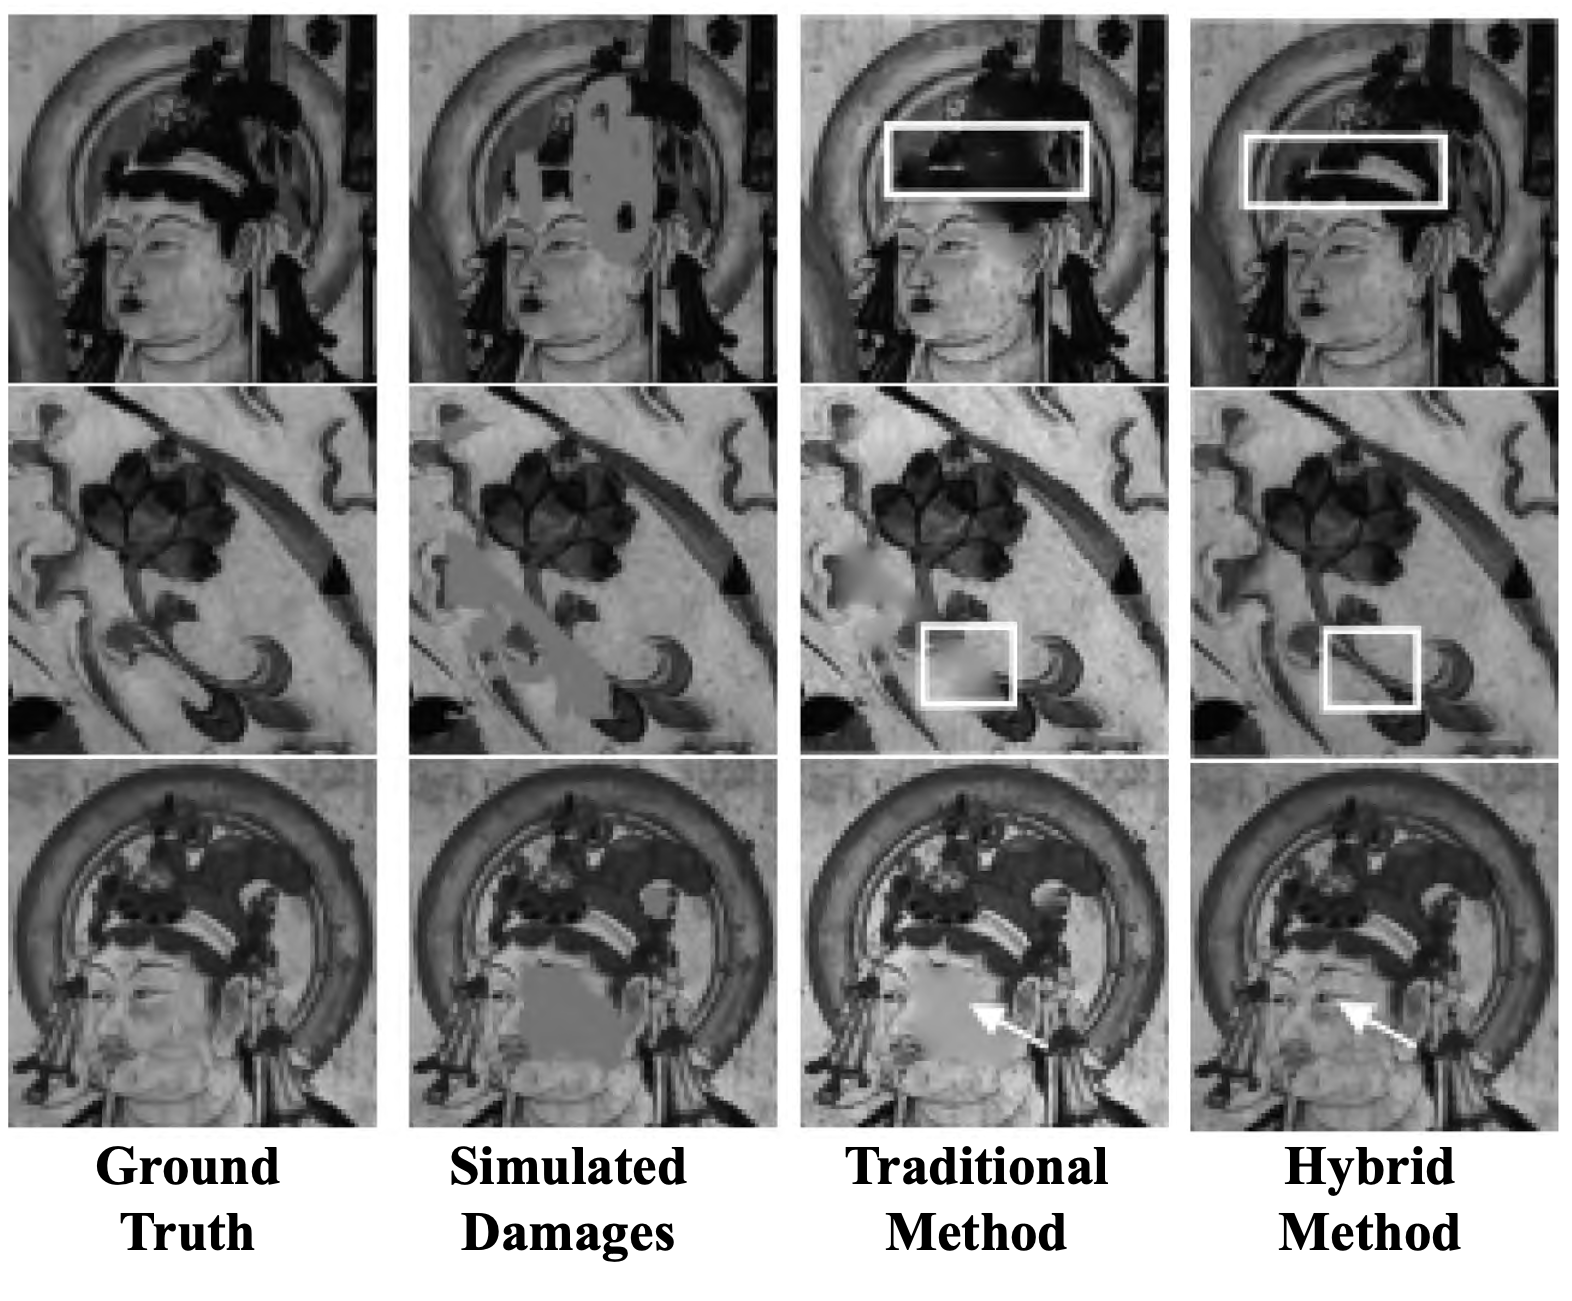
\includegraphics[width=0.6\textwidth]{figs/hybrid-method-inpainting.png}
    \end{center}

    \small\textit{Note.} Results of the hybrid image inpainting method showed satisfactory results in restoring
    complex patterns, such as the facial features of the Bodhisattva, when compared to the traditional method.
    \apacitefigfrom{Chen2024-Mural-Inpainting}
\end{figure}

\begin{figure}
    \caption{Results of the adversarial diffusion network on simulated damaged murals of complex patterns}
    \label{fig:adversarial-diffusion-inpainting}

    \begin{center}
        \includegraphics[width=0.6\textwidth]{figs/adn-inpainting.png}
    \end{center}

    \small\textit{Note.} Results of the ADN model proposed by \apaciteassub{Lian2025-Adversarial-Diffusion-Network}
    displayed advanced capabilities in restoring complex murals.
    \apacitefigfrom{Lian2025-Adversarial-Diffusion-Network}
\end{figure}

Apart from the murals, important milestones have also been achieved in the restoration of the manuscripts from
the Library Cave. The DHA has been working in collaboration with technology companies to leverage generative
artificial intelligence (GenAI) to restore and generate the missing parts of excavated manuscripts
(\apaciteaspar{Li2024-Dunhuang-Manuscripts-AIGC}). While the technical details of the algorithms are not
disclosed, it is not difficult to imagine that the approach has made use of image and text processing technologies
built on deep learning and NLP, and also the use of large datasets of calligraphy for the purpose of identifying
variants of the same Chinese characters. \apaciteassub{Li2024-Dunhuang-Manuscripts-AIGC} has remarked that
the generated contents are of promising quality and reliability. Whereas this application is still in an immature
state, it is reasonable to expect that AI technologies will gain more attention in this area.

The discussions made above focused on restoration of two-dimensional artefacts, namely the murals and manuscripts.
For three-dimensional artefacts, such as sculptures, while the use of GenAI is still in its infancy and remains
at a theoretical stage, further research on proposed methods such as that of
\apaciteassub{Ge2019-Creative-AI-Sculptural-Objects} may allow GenAI to be used for restoring damaged, if not
lost, sculptures in the Dunhuang Grottoes in the future.

Having discussed the latest advancements in the use of image inpainting and related technologies, it is conceivable
that the use of AI technologies can benefit the preservation of Dunhuang Grottoes by helping the restoration of
artefacts.

\subsection{Raising Public Awareness and Interest Through Artistic Style Transfer}

The focus of \cref{sec:automated-object-detection} and \cref{sec:image-inpainting-restoration} was on the
technical aspects of the preservation of Dunhuang's cultural heritage. However, as defined in
\cref{sec:preservation-definition}, the humanity aspect of preservation is equally important.
The key to raising public awareness and interest so as to ensure the survival of the cultural heritage
is the next generation of people. Measures for educating and inspiring the domestic (Chinese) adolescents
are distinct from those for the international audience, as they have different backgrounds. This section will
draw its focus on the former.

A new consumerism phenomenon advocating cultural identity and cultural confidence, known as the ``National Trend''
(\textit{Guochao}), has emerged in China, especially amongst the younger generation. According to
\apaciteassub{Liu2021-Guochao-Rise}, relevant queries on the Chinese search engines have increased by four times,
peaking in 2019 at 26 billion queries. Leveraging this trend is a way to promote the vibrant cultures of the
Dunhuang Grottoes, and such leverage would be made possible easily by the use of GenAI.

On the technical side, \apaciteassub{Sun2023-Dunhuang-Patterns} discussed that the use of style transfer has
long been a dominant trend in the field of artistic creation. They further stated that, however, the use of such
technology in the context of Dunhuang Arts is insufficiently explored. Trained models already exist and are capable
of producing promising results, as shown in both \cref{fig:style-transfer-showcase} and
\cref{fig:style-transfer-showcase-2}.

\begin{figure}
    \caption{Examples of results of merging Dunhuang art styles with modern images using different 
    models and algorithms}
    \label{fig:style-transfer-showcase}
    
    \begin{center}
        \includegraphics[width=0.9\textwidth]{figs/style-transfer-showcase-en.png}
    \end{center}

    \small\textit{Note.} The original figure were in Chinese. The captions are translted into English
    by the author. \apacitefigfrom{Sun2023-Dunhuang-Patterns}
\end{figure}

\begin{figure*}
    \caption{Examples of results of tranfering Dunhuang art styles onto new images by different models}
    \label{fig:style-transfer-showcase-2}

    \begin{center}
        \includegraphics[width=0.9\textwidth]{figs/style-transfer-results.png}
    \end{center}

    \small\textit{Note.} The left-most column are the original images, while the others are the results of
    Dunhuang art styles being transferred on the original images by different models.
    \apacitefigfrom{Yu2022-AI-Dunhuang}
\end{figure*}

On the public acceptance side, while no major use of GenAI in the context of Dunhuang Grottoes has been reported,
similar cases can be looked at as a reference. \apaciteassub{Zhang2023-AI-New-Year-Prints} have conducted a study
of the public's perception of the sustainability of intangible cultural heritage on AI-generated New Year products.
The results showed that the public is generally engaged and supportive of the attractive products, revealing a
positive correlation between younger generation's cultural identity and economic boost.

It is predicted that the DHA could take advantage of the current National Trend and the cutting-edge technologies,
with proper online and offline marketing strategies, to promote the Dunhuang Grottoes, as its nature of being a
valuable traditional Chinese cultural heritage is in line with the values of the National Trend and aligns with
the contemporary Chinese government's policies of promoting cultural confidence among its citizens
(\apaciteaspar{Liu2021-Guochao-Rise}). Furthermore, the DHA can borrow the experience of
\apaciteassub{Shao2023-Digital-Transformation-Dunhuang} to gain economic benefits from the market of intellectual
property, which can be used to fund the preservation work, creating a positive feedback loop.

To conclude, the use of AI technologies in artistic style transfer can be beneficial to the preservation of
the Dunhuang Buddhist heritage by raising public awareness and interest.

\section{Concerns Raised Against AI Technologies in Buddhist Heritage Preservation}

\subsection{Forfeited Authenticity and Originality in AI-Restored Artefacts}

While the algorithms and models discussed earlier have shown remarkable accuracy in the restoration of
artefacts, one must bear in mind that by no means can the AI-generated artefacts be ``authentic'' howsoever
they resemble the original. Regarding generated arts, \apaciteassub{Tiribelli2024-Ethics-AI} posed two 
critical questions regarding the authorship and whether the generated art is eligible to be claimed as
``original'' or ``authentic''.

While authorship is not within the scope of discussion of this paper, the authenticity, however, is difficult to guarantee.
As discussed earlier, GenAI relies on the datasets on which they were trained. Even if the algorithms were designed
to be absolutely neutral, which only exist in an ideal condition, the dataset can already be comprimised with bias
of which the developers are not aware of. Plus, since it is inevitable to have an imbalance in the number of
available data amongst different categories of data, AI models tend to misinterpret parts on which they were not
adequately trained. \apaciteassub{Fu2025-AI-Intangible-Cultural-Heritage} mentioned an incident of an AI model
empolyed by the Shanghai Digital Heritage Centre misinterpreting Tibetan cultural elements due to the fact that
it was trained predominantly on the cultures of the Han dynasty. It is therefore inferred that contemporary AI
technologies are not yet reliable in terms of authenticity.

Even if the authenticity can be guaranteed in a hypothetical scenario, one must recognise that ``authenticity''
and ``originality'' are two distinct concepts. \apaciteassub{Li2022-AI-Restoration-Copyright} mentions two types
of authenticity -- moral authenticity and type authenticity, which asserts the AI models' ability to extract the
artist's intentions from the style of the original artefacts. The ability to extract qualifies the AI-generated
artefacts to be ``authentic'', as they were created with the original artist's process of thoughts, however by no
means be ``original''. It comes naturally that one would argue that the AI-generated or -restored artefacts forfeit
their authenticity, if not originality.

If such originality issue is not addressed, although the application of AI technologies advantages the technical
aspect of preservation, it may undermine the message conveyed by the artefacts, which in turn comprimises the
humanity aspect of preservation. As of the case of Dunhuang Grottoes, the restored artefacts proposed by
\apaciteassub{Yu2022-AI-Dunhuang} and \apaciteassub{Lian2025-Adversarial-Diffusion-Network} are not currently
displayed for the general public, but rather for research purposes only. Therefore, the Dunhuang Grottoes are
not in immediate risk of forfeiture of authenticity and originality, but thorough assertions must be made
before an official endorsement can be made.

\subsection{Misinformation and Hallucination of LLMs}

It is of common knowledge that LLMs are prone to generating misinformation, or having hallucinations when they
attempt to generate output in a less familiar area. This behaviour is rooted in the way LLMs produce output,
thus inevitable (\apaciteaspar{Saha2025-LLM-Hallucination}).

In particular, in the context of Dunhuang Grottoes,
the LLMs are expected to provide service in a field that is highly specialised and requires expertise. Frankly,
as \apaciteassub{Shen2024-LLM-History-Education} have shown, despite the unrivalled mastery of languages,
LLMs are falling short in terms of knowledge in the field of seconary-education-level history, let alone the
specialised knowledge in the field of archaeology and Buddhist history. The research by
\apaciteassub{Jiang2024-Digital-Dunhuang} also backs this claim, that is, there exists a high potential for LLMs
to provide incorrect information when prompted.

While measures have been proposed to combat this issue, such as using multiple layers of LLMs to verify the 
reliability of the output
(\apaciteaspar{Saha2025-LLM-Hallucination}; \apaciteaspar{Verspoor2024-LLM-Hallucination}),
the application of such error-prone technologies to provide public education remains a concerning risk
of comprimising the purpose of preservation.

\section{Conclusion}

\printbibliography